\documentclass{article}
\usepackage[utf8]{inputenc}
\usepackage{fullpage}
\usepackage{amsmath}
\usepackage{graphicx}
\usepackage{amsfonts}
\usepackage{mathrsfs} 
\usepackage{float}
\usepackage[ruled,vlined]{algorithm2e}
\usepackage{url}
\newcommand*\mean[1]{\bar{#1}}
\usepackage{amsthm}


\title{Optimización con restricciones PDE's}

\begin{document}
\theoremstyle{definition}
\newtheorem{definition}{Definición}[section]
\newtheorem{theorem}{Teorema}
\newtheorem*{definition*}{Definición}
\newtheorem*{theorem*}{Teorema}

\maketitle

\noindent
Queremos resolver problemas del estilo 
\begin{equation}
\begin{split}
    &\min_{w\in W}J(y,u)\\
    \text{ s.t. } &e(y,u)=0, c(y,u)\in \mathcal{K},w\in\mathcal{C}
\end{split}
\end{equation}
donde $J:\mathcal{W}=\mathcal{Y}\times\mathcal{U}\to \mathbb{R}$ es la función objetivo, $e:\mathcal{W}\to \mathcal{Z}$ y $c:\mathcal{W}\to \mathcal{R}$ son operadores entre espacios de Banach reales $\mathcal{W},\mathcal{Z},\mathcal{R}$, además $\mathcal{K}\subset \mathcal{R}$ es un cono convexo cerrado y $\mathcal{C}\subset\mathcal{W}$ es un conjunto cerrado convexo.  En general, los espacios considerados son espacios de funciones que son soluciones débiles a ecuaciones diferenciales parciales asociadas al operador $e(y,u)$, donde esta ecuación describe un sistema con función de estado $y$ y control $u$.\\

\noindent
La solución de este tipo de problemas se hace necesaria en diversos contextos, de los cuales escogemos uno particular para ilustrar de manera sencilla la teoría y los métodos numéricos a usar . Supongamos que tenemos un cuerpo sólido definido en un dominio $\Omega\subset\mathbb{R}^3$ acotado, cuya temperatura en determinado instante es descrita por la función $y(x)$. Queremos que la distribución de temperatura de este cuerpo sea lo más parecida posible a una distribución dada $y_d(x)$, para lo cual vamos a modelar el problema mediante el siguiente problema de optimización
\begin{equation}
\label{prom2}
    \begin{split}
        \min J(y,u)=\frac{1}{2}\int_{\Omega}&(y(x)-y_d(x))^2dx+\frac{\lambda}{2}\int_{\Omega}u(x)^2dx\\
        \text{s.t.  }& -\Delta y=\beta u \text{ en } \Omega\\
        &y=0 \text{  en   }\partial\Omega.\\
        u_a(x)&\leq u(x)\leq u_b(x) \text{ casi siempre}
    \end{split}
\end{equation}
En este modelo, $u$ representa una variable de control, que es la que se puede modificar en el problema físico. La primera restricción es la ecuación de calor estacionaria que debe cumplir la distribución de temperatura, la segunda  representa las condiciones de frontera que debe cumplir la distribución de temperatura, y por simplicidad se toman condiciones de Dirichlet. Se modela la distancia de la distribución de de temperatura $y$ a la deseada $y_d$ mediante el primer termino del funcional $J$, usando para ello la norma en $L_2(\Omega)$, y además se agrega el segundo termino que sirve para regularizar el problema y cuenta como el que se tiene al ejercer el control $u$ en el dominio. Además, podemos incluir la restricción en la que el control elegido este entre dos funciones dadas en $L_2(\Omega).$\\
\section{Ecuaciones Diferenciales parciales}
Para establecer resultados de optimalidad, será necesario desarrollar primero resultados de existencia, para lo cual se requiere de la teoría de ecuaciones en derivadas parciales. A continuación se presentan algunas definiciones y resultados útiles sin demostración que serán usados posteriormente.\\

\noindent
A lo largo de todo el documento se considera que un dominio es un abierto conexo de $\mathbb{R}^n$, y serán denotados por $\Omega$. Para la existencia de soluciones de ecuaciones en derivadas parciales se requiere cierta regularidad en el dominio considerado. Aquí serán considerados suficientes los dominios de Lipschitz, en los cuales cada punto $x$  de la frontera del dominio $\partial\Omega$ está contenido en un abierto $U_x$ tal que  $U_x\cap \partial\Omega$ es la imagen de una función Lipschitz continua.\\

\noindent
Por lo general, los problemas del mundo real no permiten soluciones a ecuaciones en términos del sentido clásico de derivabilidad, por lo que hay que extender este concepto para obtener espacios de soluciones suficientemente grandes. 


\iffalse
En los dominios de Lipschitz acotados el teorema de Gauss es válido, por lo que para $y,v\in C^1(\overline{\Omega})$ tenemos la formula de integración por partes
\begin{equation*}
    \int_{\Omega}v(x)D_iy(x)dx=\int_{\Gamma}v(x)y(x)\nu_i(x)ds(x)-\int_{\Omega}y(x)D_iv(x)dx,
\end{equation*}
en donde $\nu_i$ es la $i$-ésima componente vector unitario normal $\nu(x)$ a $\Gamma$, la frontera del dominio, en el punto $x$. En particular, si $v(x)=0$ en $\Gamma$ se tendría
\begin{equation*}
    \int_{\Omega}y(x)D_iv(x)dx=-\int_{\Omega}v(x)D_iy(x)dx
\end{equation*}
Y en general, para $y\in C^k(\overline{\Omega}), v\in C_0^k(\overline{\Omega})$, y cualquier multi-indice $\alpha$ con $|\alpha|<k$, se tiene
\begin{equation*}
    \int_{\Omega}y(x)D^\alpha v(x)dx=(-1)^{|\alpha|} \int_{\Omega}v(x)D^\alpha y(x)dx
\end{equation*}
\fi

\noindent
Motivado en las formula de integración por partes multidimensional que proporciona el teorema de Gauss aplicada a funciones con soporte compacto en $\overline{\Omega}$ definimos
\theoremstyle{definition}
\begin{definition}
Sea $y\in L_{loc}^1(\Omega)$, donde $L_{loc}^1(\Omega)$ es el espacio de funciones localmente integrables en $\Omega$,  y $\alpha$ un multi-indice dado. Si una función $w\in  L_{loc}^1(\Omega)$ satisface $\forall v\in C_0^{\infty}(\Omega)$
\begin{equation}
    \int_{\Omega}y(x)D^\alpha v(x)dx=(-1)^{|\alpha|} \int_{\Omega}w(x)v(x)dx
\end{equation}
entonces $w$ es llamada la derivada débil de $y$ asociada a $\alpha$
\end{definition}

\theoremstyle{definition}
\begin{definition}
Sea $1\leq p<\infty$. Definimos el espacio de Sobolev $W^{k,p}(\Omega)$ como el espacio de funciones $y\in \L^p(\Omega)$ con derivadas débiles $D^{\alpha}y$ en $L^p(\Omega)$ para todos los multi-indices $\alpha$ con $|\alpha|\leq k$, dotado con la norma
\begin{equation}
    ||y||_{W^{k,p}(\Omega)}=\left(\sum_{|\alpha|\leq k}\int_{\Omega}|D^\alpha y(x)|^pdx\right)^\frac{1}{p}
\end{equation}
Para el caso especial $p=2$, denotamos $H^k(\Omega):=W^{k,2}(\Omega)$
\end{definition}

\noindent
Se tiene que estos espacios son de Banach, y para el caso $p=2, k=1$ se puede dotar de producto interno que genera la norma definido por 
\begin{equation}
    (u,v)_{H^1(\Omega)}=\int_{\Omega}uvdx+\int_{\Omega}\nabla u\cdot \nabla v dx,
\end{equation}
convirtiéndolo en espacio de Hilbert.
\theoremstyle{definition}
\begin{definition}
La clausura de $C_0^{\infty}(\Omega)$ en $W^{k,p}(\Omega)$ es denotada por $ W_0^{k,p}(\Omega)$ y además para $p=2$ se denota $H_0^2(\Omega):=W_0^{k,2}(\Omega)$. Puede considerarse como el espacio de funciones que, junto con sus derivadas débiles hasta orden $k-1$, se anulan en la frontera de $\Omega$.
\end{definition}

\noindent
Estamos interesados en resolver problemas de la ecuación de Poisson con condiciones de frontera de Dirichlet, que son del estilo 
\begin{equation}
\label{eqn:Posiion}
    \begin{split}
        -\Delta &y=u\\
        y&=0 \text{ en } \partial\Omega
    \end{split}
\end{equation}
donde $u\in L_2(\Omega)$. Dado que $u$ puede ser muy irregular, la existencia de soluciones en $C^2(\Omega)\cap C(\bar{\Omega})$ no está garantizada, por lo que hemos de buscar soluciones en $H_0^1(\Omega)$. Para este fin, consideremos que $u$ es lo suficientemente regular para permitir soluciones clásicas $y\in C^2(\Omega)\cap C(\bar{\Omega})$, multiplicando la ecuación de Poisson por una función test arbitraria $v\in C_0^{\infty}(\Omega)$ e integrando sobre $\Omega$ obtenemos 
\begin{equation}-\int_{\Omega} v \Delta y d x=\int_{\Omega} f v d x\end{equation}
de donde, usando integración por partes multidimencional, concluimos que
\begin{equation}-\int_{\Gamma} v \nabla y\cdot\nu d s+\int_{\Omega} \nabla y \cdot \nabla v d x=\int_{\Omega} f v d x\end{equation}
denotando $\nu$ el vector normal unitario a $\partial \Omega$. Además, como $v$ se anula en $\partial \Omega$, se obtiene que para toda $v\in C_0^{\infty}(\Omega)$
\begin{equation}\int_{\Omega} \nabla y \cdot \nabla v d x=\int_{\Omega} f v d x.\end{equation}
En particular, como esta condición vale para toda $v\in C_0^{\infty}(\Omega)$, las expresiones dependen continuamente de $v$ y $C_0^{\infty}(\Omega)$ es denso en $H_0^{1}(\Omega)$, entonces vale también para cualquier $v\in H_0^{1}(\Omega)$. Además, es posible mostrar que cualquier $y\in H_0^{1}(\Omega)$ que satisfaga esta relación para cualquier $v \in C_0^{\infty}(\Omega)$ y que sea lo suficientemente suave, es también solución del problema clásico. Esto motiva la definición

\theoremstyle{definition}
\begin{definition}
Decimos que $y\in H_0^{1}(\Omega)$ es una solución débil al problema  \ref{eqn:Posiion} si satisface la llamada formulación débil o variacional. 
\begin{equation}\int_{\Omega} \nabla y \cdot \nabla v d x=\int_{\Omega} f v d x \quad \forall v \in H_{0}^{1}(\Omega)\end{equation}
Notemos que la condición de frontera ya está implícita en esta relación.
\end{definition}

\noindent
Para escribir este problema de una forma más compacta, definamos la función bilineal $a:H_{0}^{1}\times H_{0}^{1}\to \mathbb{R}$ como 
\begin{equation}a[y, v]=\int_{\Omega} \nabla y \cdot \nabla v d x\end{equation}, que se puede mostrar define un producto interno en $H_{0}^{1}$,
y el funcional $F:H_{0}^{1}(\Omega) \to \mathbb{R}$ como 
\begin{equation}
F(v)=\int_{\Omega}fv dx=(f, v)_{L^{2}(\Omega)}.
\end{equation} 
De esta manera, el problema se resume en encontrar $y\in H_{0}^{1}(\Omega)$ para el cual $a[y,v]=F(v)$ para toda $v\in H_{0}^{1}(\Omega) $.\\

\noindent
La existencia de soluciones débiles para la ecuación de Poisson con condiciones de frontera de Dirichlet se justifica mediante los siguientes teoremas del análisis funcional.

\begin{theorem}[Teorema de representación de Riesz]
Para todo funcional lineal acotado $F:\mathcal{H}\to \mathbb{R}$ en un espacio de Hilbert $\mathcal{H}$, hay un único elemento $y\in \mathcal{H}$ tal que $F(v)=(v,y)$ para todo $v\in \mathcal{H}$. Además, la norma del funcional $F$ concuerda con la norma de $y$.
\end{theorem}

\begin{theorem}[Desigualdad de Poincaré]
Si $\Omega\subset\mathbb{R}^n$ es un dominio acotado, entonces existe una constante $C=C(\Omega)$ dependiente solo del dominio tal que 
\begin{equation}
    \int_{\Omega}|v(x)|^2 dx \leq C\int_{\Omega}|\nabla v(x)|^2 dx
\end{equation}
para todo $v\in H_{0}^{1}(\Omega) $
\end{theorem}

\noindent
Con estos resultados, es posible asegurar la existencia de soluciones débiles para el problema original, pues tomando $\mathcal{H}=H_{0}^{1}(\Omega)$, nuestro funcional $F$ es acotado ya que  $f\in L_2(\Omega)$, $v\in H_{0}^{1}(\Omega)$ y además
\begin{equation}
    |F(v)|=\left|\int_{\Omega}fvdx\right|\leq ||f||_2||v||_2\leq\sqrt{C}||f||_2 \sqrt{a[v,v]},
\end{equation}
donde se usó la desigualdad de Cauchy-Schwarz y la desigualdad de Poincaré. Por lo tanto, aplicando el teorema de representación de Riesz, obtenemos la existencia y unicidad de soluciones débiles para el problema \ref{eqn:Posiion}.\\


\noindent
Para problemas más generales es necesario desarrollar otros teoremas de existencia, de entre ellos el más relevante es el teorema de Lax-Milgram. Sin embargo, la teoría desarrollada es suficiente para lo que sigue.
\section{Teoría de optimalidad}
Recordemos que si $U$ y $V$ son espacios de Banach, entonces $\mathcal{L}(U,V)$ denota el espacio de todos los mapeos lineales continuos de $U$ a $V$ dotado con la norma $|f|=\sup_{|u|=1}|f(u)|$. El espacio $U^{*}=\mathcal{U,\mathbb{R}}$ es denominado el dual de $U$ y consiste de los funcionales lineales continuos en $U$.\\

\noindent
Ahora, sea $U$ un espacio de Banach y $U^{*}$ su dual, consideremos un $u\in U$ fijo  y el mapa inducido por este elemento en $U^{*}$ dado por $F_u:U^{*}\to \mathbb{R}$ que actúa como $F_u(f)=f(u)$. Tenemos que este funcional es lineal y acotado en $U^{*}$, por lo que pertenece al dual de $U^{*}$, llamado el bidual de $U$ y denotado por $U^{**}$. Como el mapa $u\to F_u$ es inyectivo, podemos identificar $u$ con $F_u$, interpretando así a $u\in U$ como un elemento en $U^{**}$. Al anterior mapa se denomina el embebimiento canónico de $U$ en $U^{**}$, si este mapa es además sobreyectivo, entonces $U=U^{**}$ y decimos que $U$  es reflexivo. El teorema de representación de Riesz establece una correspondencia biyectiva isométrica entre un espacio de Hilbert y su dual, por lo que todo espacio de Hilbert es isométricamente isomorfo a su bidual, por lo que todo espacio de Hilbert es reflexivo.\\

\noindent
Para probar la existencia de óptimos para el problema $\ref{problema}$ debemos establecer algunas definiciones y resultados previos del análisis funcional.
\theoremstyle{definition}
\begin{definition}
Sea $U$ un espacio de Banach, se dice que una succesión $\{u_n\}_{n=1}^{\infty}\subset U$ es debilmente convergente a algún $u\in U$ si para todo $f\in U^{*}$ se tiene que $\lim_{n\to \infty}f(u_n)=f(u)$, y en este caso se denota $u_n\rightharpoonup u$.
\end{definition}
\theoremstyle{definition}
\begin{definition}
Sean $U$ y $V$ espacios de Banach. Un mapa $F:U\to V$ se dice debilmente secuencialmente continuo si para toda sucesión $\{u_n\}_{n=1}^{\infty}\subset U$ tal que converja débilmente a un $u\in U$, entonces su imagen  $\{F(u_n)\}_{n=1}^{\infty}\subset V$ converge debilmente a $F(u)$ en $V$.  Es decir $u_n\rightharpoonup u \implies F(u_n)\rightharpoonup F(u)$
\end{definition}
\theoremstyle{definition}
\begin{definition}
Sea $M\subset U$ un subconjunto de un espacio de Banach. Decimos que $M$ es débilmente secuencialmente cerrado si el limite de toda sucesión débilmente convergente está en M. Además, M es débilmente secuencialmente relativamente compacto si toda sucesión $\{u_n\}_{n=1}^{\infty} \subset M$ contiene una sub-sucesión débilmente convergente, y si $M$ es débilmente secuencialmente cerrado, entonces decimos que $M$ es débilmente secuencialmente compacto.
\end{definition}

\begin{theorem}
Todo conjunto acotado de un espacio de Banach reflexivo es débilmente secuencialmente relativamente compacto.
\end{theorem}

\begin{theorem}
Todo conjunto convexo y cerrado en un espacio de Banach es débilmente secuencialmente cerrado. Si el espacio es reflexivo y el conjunto es acotado, entonces el conjunto es débilmente secuencialmente compacto.
\end{theorem}

\begin{theorem}
Todo funcional $f:U\to \mathbb{R}$ continuo y convexo en un espacio de Banach es débilmente semicontinuo por abajo. Es decir,  para cualquier sucesión $\{u_n\}_{n=1}^{\infty} \subset U$ debilmente convergente a $u$ se tiene que $\liminf f(u_n)\geq f(u)$
\end{theorem}

\noindent
Podemos usar estos resultados para establecer resultados de problemas de optimalidad del tipo 
\begin{equation}
\label{prom}
    \begin{split}
        \min J(y,u)=\frac{1}{2}\int_{\Omega}&(y(x)-y_d(x))^2dx+\frac{\lambda}{2}\int_{\Omega}u(x)^2dx\\
        \text{s.t.  }& -\Delta y=\beta u \text{ en } \Omega\\
        &y=0 \text{  en   }\partial\Omega.\\
        u_a(x)&\leq u(x)\leq u_b(x) \text{ casi siempre}
    \end{split}
\end{equation}
donde $\Omega$ es un dominio Lipschitz, $\lambda\geq 0$, $y_d,u_a,u_b\in L_2(\Omega)$, $\beta\in L_{\infty}(\Omega)$ y $u_a\leq u_b$ casi siempre. \\

\noindent
Para solucionar este problema primero se debe elegir el espacio de control al  cual va a pertenecer la solución $u$. Una elección razonable viene dada por $U_{ad}=\{u\in L_2(\Omega): u_a(x)\leq u(x) \leq u_b(x)\text{ casi siempre }\}$ , que es un conjunto no vacio, cerrado y convexo de $L_2(\Omega)$. Para cada control admisible en este espacio, por el teoría desarrollada en la sección anterior, existe una solución débil $y\in H_{0}^{1}(\Omega)$ al problema de valor en la frontera considerado, esta solución se denomina el estado asociado a $u(x)$ y se denomina a $H_{0}^{1}(\Omega)$ como el espacio de estados.

\begin{definition}
Llamamos a un control admisible $\bar{u} \in U_{ad}$ un control óptimo y su correspondiente estado asociado $\bar{y}\in H_{0}^{1}(\Omega)$ el estado óptimo si $J(\bar{u},\bar{y})\leq J(y(u),u)$ para todo $u \in U_{ad}$.
\end{definition}

\noindent
Denotamos por $G:L_2(\Omega)\to H_{0}^{1}(\Omega)$ el operador que asocia a cada $u\in L_2(\Omega)$ la correspondiente solución de problema de valor en la frontera y lo llamamos el operador control-a-estado. Además como podemos embeber $H^1(\Omega)$ en $L_2(\Omega)$ continuamente, podemos considerar el operador $SL_2(\Omega)\to L_2(\Omega)$ que asocia a cada $u\in L_2(\Omega)$ con la correspondiente solución $y$ embebida en $L_2(\Omega)$.\\

\noindent
Tenemos el siguiente resultado de existencia de óptimos para el problema \ref{prom}.

\begin{theorem}
Sean $U,\mathcal{H}$ espacios de Hilbert, y sea $U_ad\subset U$ un subespacio no vacio, cerrado, acotado y convexo de $U$. Además, sean $y_d\in \mathcal{H}$, $\lambda\geq 0$ y $S:U\to \mathcal{H}$ un operador lineal acotado. Entonces el problema 
\begin{equation}
    \min_{u\in U_{ad}}f(u)=\frac{1}{2}||Su-y_d||_{\mathcal{H}}^2+\frac{\lambda^2}{2}||u||_{U}^2
\end{equation}
admite una solución óptima $\bar{u}\in U_ad$. Si $\lambda>0$ o $S$ es inyectiva entonces la solución es única.
\end{theorem}
\begin{proof}
Tenemos que $f(u)\geq 0$ para todo $u\in U_{ad}$, luego el conjunto es acotado y existe un ínfimo
\begin{equation*}
    j=\inf_{u\in U_{ad}}f(u)
\end{equation*}
y existe una sucesión $\{u_n\}_{n=1}^{\infty} \subset U_{ad}$ tal que $f(u_n)\to j$ cuando $n\to \infty$. Tenemos además que $U_{ad}$ es cerrado y acotado, luego por el teorema 4 de esta sección, el conjunto es débilmente secuencialmente compacto dado que es un espacio de Hilbert y por lo tanto reflexivo. Por lo tanto, existe una sub-sucesión $\{u_{n_k}\}_{k=1}^{\infty}$ que converge débilmente a algún $\bar{u}\in U_{ad}$. Por otro lado, dada la continuidad de $S$, tenemos que el funcional $f$ es continuo, además es convexo y luego por el teorema 5 es débilmente semi-continuo por abajo, por lo tanto $f(\bar{u})\leq \liminf_{k\to \infty} f(u_{n_k})=j$. Como $\bar{u}\in U_{ad}$, se debe tener $f(\bar{u})=j$ y por lo tanto es un control óptimo. La unicidad viene de la convexidad estricta en el caso en que $\lambda>0$ o $S$ sea inyectivo.
\end{proof}

\noindent
Notemos que en la prueba solo fue necesario que $f$ fuera continuo y convexo, y que $U$ fuera reflexivo, pudiéndose usar el resultado en los casos en los que esto se cumpla.\\

\noindent
Podemos usar este teorema para asegurar la existencia de un óptimo para el problema \ref{prom}, y obtendríamos su unicidad en el caso en que $\lambda>0$ o bien $b\neq 0$. En el caso en que $u_a(x)=-\infty$ o $u_b(x)=\infty$, el conjunto $U_{ad}$ ya no es acotado, sin embargo, también se puede mostrar existencia y unicidad cuando $\lambda>0$.\\

\noindent
Una vez comprobada la existencia y posible unicidad, vamos a caracterizar el óptimo $\bar{u}$ para este tipo de problemas con analogías al caso finito, encontrando condiciones de primer orden que sean útiles para encontrar dichos óptimos. Para ello, recordemos que se puede definir una noción de derivada en espacios más generales mediante las derivada de Gateaux y Frechet trabajadas al comienzo del curso.\\

\begin{definition}
Sean $u,h\in U$ dados, y sea $F:U\to V$ , con $U$ y $V$ espacios de Banach, si el limite
\begin{equation}\delta F(u, h):=\lim _{t \downarrow 0} \frac{1}{t}(F(u+t h)-F(u))\end{equation}
existe en $V$, entonces es llamado la derivada direccional de $F$ en $u$ en la dirección $h$. Si el limite existe para todo $h\in U$, entonces el mapeo $h\to \delta F(u,h)$ se denomina primera variación de $F$ en $u$. Si existe un operador lineal continuo $A:U\to V$ tal que $\delta F(u,h)=Ah$ para todo $h\in U$, entonces $F$ se dice Gateaux derivable en $u$ y se denota por $F'(u)=A$ su derivada.
\end{definition}

\noindent
Para nosotros va a ser importante calcular la derivada del funcional $f:\mathcal{H}\to \mathbb{R}$ dado por $f(u)=||u||_{\mathcal{H}}^2$. Tenemos que \begin{equation*}\begin{aligned}
\lim _{t \rightarrow 0} \frac{1}{t}(f(u+t h)-f(u)) &=\lim _{t \rightarrow 0} \frac{1}{t}\left(\|u+t h\|_{\mathcal{H}}^{2}-\|u\|_{\mathcal{H}}^{2}\right) 
&=\lim _{t \rightarrow 0} \frac{2 t(u, h)_{\mathcal{H}}+t^{2}\|h\|_{\mathcal{H}}^{2}}{t} 
&=2(u, h)_{\mathcal{H}}
\end{aligned}\end{equation*}
luego $f'(u)h=(2u,h)$, e identificando $\mathcal{H}$ con su dual por medio del teorema de representación de Riesz tendríamos $f'(u)=2u$, denominado el gradiente de $f$ en $u$.

\begin{definition}
Decimos que $F$ es Frechet diferenciable si existe un operador lineal $A:U\to V$ tal que
\begin{equation}\frac{\|F(u+h)-F(u)-A h\|_{V}}{\|h\|_{U}} \rightarrow 0 \quad \text { cuando }\|h\|_{U} \rightarrow 0\end{equation}
\end{definition}

\noindent 
Tenemos además, de forma informal, que se puede derivar composiciones del estilo $E(u)=G\circ F(u)=G(F(u))$ usando la regla de la cadena siempre y cuando $F$ y $G$ sean Frechet diferenciables. Vamos a querer calcular la derivada del operador $E(u)=||Su-z||_{\mathcal{H}}^2$, que es la composición de $G(v)=||v||_{\mathcal{H}}^2$ y $F(u)=Su-z$, luego, usando la regla de la cadena obtenemos que $E'(u)h=G'(F(u))F(u)h=2(Su-z,Sh)_{\mathcal{H}}=2(S^{*}(Su-z),h)_{U}$, donde $S^{*}$ es el operador adjunto tradicional, por lo tanto, hemos calculado el gradiente de $E$ en $u$, resultando en $E'(u)=2S^{*}(Su-z)$.\\

\noindent
Recordemos el siguiente resultado de optimalidad asociado a condiciones de primer orden que habíamos visto antes
\begin{theorem}
Sea $C$ un subespacio no vacio convexo de un espacio de Banach $U$, y sea $f$ un mapa Gateaux diferenciable en un abierto que contiene a $C$. Si $\bar{u}\in C$ es una solución al problema $\min_{u\in C}f(u)$, entonces cumple la desigualdad variacional $f'(u)(u-u')\geq 0$ para todo $u\in C$. Reciprocamente, si $\bar{u}\in C$ cumple esta desigualdad siempre y $f$ es convexa, entonces $\bar{u}$ es una solución al problema de minimización.
\end{theorem}

\begin{theorem}
En el contexto del teorema 6, una $\bar{u}\in U_{ad}$ es una solución al problema de minimización si y solo si cumple la desigualdad variacional
\begin{equation}\left(S^{*}\left(S \bar{u}-y_{d}\right)+\lambda \bar{u}, u-\bar{u}\right)_{U} \geq 0 \quad \forall u \in U_{a d}\end{equation}
\end{theorem}
\begin{proof}
Usamos lo que hemos calculado para concluir que el gradiente del funcional es $f'(\bar{u})=S^{*}(S\bar{u}-y_d)+\lambda \bar{u}$, luego la desigualdad es consecuencia directa del teorema 7.
\end{proof}

\noindent
Para aplicar estos resultados al problema \ref{prom}, es necesario conocer una forma explícita del operador adjunto $S^{*}$, para lo cual tenemos lo siguiente

\begin{theorem}
Sean $z,u\in L_2(\Omega)$ y $c_0, \beta \in L_{\infty}(\Omega)$ con $c_0(x)\geq 0$ casi siempre en $\Omega$. Sean $y,p\in H_{0}^{1}(\Omega)$ las soluciones débiles a los problemas 
\begin{equation}\begin{aligned}
-\Delta y+c_{0} y &=& \beta u & & \text{ en } \Omega \\
y &=& 0 & & \text{ en } \partial\Omega
\end{aligned}\end{equation}
y 
\begin{equation}\begin{aligned}
-\Delta p+c_{0} p &=& z & & \text { en } \Omega \\
p &=& 0 & & \text { en } \partial \Omega .
\end{aligned}\end{equation}
Entonces 
\begin{equation}\int_{\Omega} z y d x=\int_{\Omega} \beta p u d x\end{equation}
\end{theorem}
\begin{proof}
Multiplicando por la función test $p\in H_{0}^{1}(\Omega)$ e integrando en el primer problema, y multiplicando por la función test $y\in H_{0}^{1}(\Omega)$ e integrando en el segundo problema obtenemos
\begin{equation*}
\begin{split}
    \int_{\Omega}\left(\nabla y \cdot \nabla p+c_{0} y p\right) d x&=\int_{\Omega} \beta p u d x\\
    \int_{\Omega}\left(\nabla p \cdot \nabla y+c_{0} p y\right) d x&=\int_{\Omega} z y d x
\end{split}\end{equation*}
Como ambos lados izquierdos son iguales, los lados derechos también lo son.
\end{proof}

\begin{theorem}
Para el problema de valor en la frontera 
\begin{equation}\begin{aligned}
-\Delta y &=& \beta u & & \text { en } \Omega \\
y &=& 0 & & \text { en } \partial \Omega .
\end{aligned}\end{equation}
El adjunto del operador $S:L_2(\Omega)\to L_2(\Omega) $ control-a-estado, $S^{*}$ viene dado por 
\begin{equation*}
    S^{*}z=\beta p
\end{equation*}
donde $p\in H_{0}^{1}(\Omega)$ es la solución débil al problema 
\begin{equation}\begin{aligned}
-\Delta p &=& \beta z & & \text { en } \Omega \\
p &=& 0 & & \text { en } \partial \Omega .
\end{aligned}\end{equation}
\end{theorem}
\begin{proof}
Los operadores adjuntos en los espacios de Hilbert están caracterizados por la igualdad
\begin{equation*}(z, S u)_{L^{2}(\Omega)}=\left(S^{*} z, u\right)_{L^{2}(\Omega)} \quad \forall z \in L^{2}(\Omega), \quad \forall u \in L^{2}(\Omega)\end{equation*}
Por el teorema 9, eligiendo $c_0=0$ y $y=Su$ tenemos que
\begin{equation*}(z, S u)_{L^{2}(\Omega)}=(z, y)_{L^{2}(\Omega)}=(\beta p, u)_{L^{2}(\Omega)}\end{equation*}
el teorema de existencia de soluciones para este tipo de problemas desarrollado en el anterior sección provee que el mapeo $z\to \beta p$ es lineal y continuo de $L_2(\Omega)$ en sí mismo. Como $z$ y $u$ se pueden escoger arbitrariamente y $S^{*}$ está únicamente determinado, concluimos que $S^{*}z=\beta p$. 
\end{proof}

\noindent
Con esto obtenemos una caracterización para el gradiente del funcional $f$ en el problema $\ref{prom}$, dada por $f'(u)=p +\lambda u$, donde $p$ satisface el problema de valor en la frontera
\begin{equation}\begin{aligned}
-\Delta p &= Su -y_d &  \text { en } \Omega \\
p &= 0 &  \text { en } \partial \Omega .
\end{aligned}\end{equation}
lo cual es suficiente para implementar un método numérico que lo resuelva, lo cual se hará a continuación.\\

\noindent
Obtener como actúa el operador adjunto $S^{*}$ para otro tipo de problemas puede ser más complicado. Sin embargo, existe un método heurístico que utiliza la función lagrangiana asociada al problema de optimización que permite calcularlo fácilmente, pero dada la extensión que podría alcanzar el documento si la incluyo prefiero conformarme con lo ya hecho y obtener resultados numéricos a partir de ello.

\section{Métodos Numéricos}
Para ilustrar algunos métodos que pueden ser usados para resolver el problema de optimización tratado, vamos a resolver el problema especifico
\begin{equation}
\label{prom3}
    \begin{split}
        \min J(y,u)=\frac{1}{2}\int_{\Omega}&(y(x)-y_d(x))^2dx+\frac{\lambda}{2}\int_{\Omega}u(x)^2dx\\
        \text{s.t.  }& -\Delta y=\beta u \text{ en } \Omega\\
        &y=0 \text{  en   }\partial\Omega.\\
    \end{split}
\end{equation}
donde $\Omega=[0,1]\times [0,1]$, $\beta=1 $, $\lambda=0.1$ y $y_d$ se elige como la distribución de temperatura que se obtiene cuando se aplica el control $u=e^{-(x-0.5)^2-(y-0.5)^2}$.
\subsection{Primero optimizar, luego discretizar}
Este tipo de métodos consiste en usar la información descubierta anteriormente de la estructura del espacio y las condiciones de primer orden para optimalidad. En particular, podemos usar la caracterización dada del gradiente para implementar métodos como el descenso del gradiente tradicional que sigue funcionando en los espacios considerados , el algoritmo implementado para este problema se resume en lo siguiente\\

\begin{algorithm}[H]
\SetAlgoLined
\KwResult{Óptimo del problema planteado}
 Elija $u_0\in L_2(\Omega)$, $\alpha\in (0,1)$ \;
 \While{$||\nabla f(u_k)||_{L_2(\Omega)}>\epsilon$}{
  Resuelva el problema $-\Delta y_k=u_k$ con las condiciones de frontera impuestas\;
  Resuelva el problema $-\Delta p=y_k-y_{d}$\ con las condiciones de frontera impuestas;
  $u_{k+1}=u_{k}-\alpha(\lambda u_k + p)$
 }
 \caption{Descenso del gradiente}
\end{algorithm}
\noindent
En cada iteración del algoritmo es necesario resolver la ecuación de Poisson con condiciones de frontera de Dirichlet, para lo cual se discretiza el problema, en este caso con un esquema en diferencias finitas, aunque también podría realizarse con algún otro tipo de discretización. El sistema resultante se resuelve con el paquete de matrices dispersas de scipy. En la implementación se discretizó el dominio con una malla de $50\times 50$ puntos. Para calcular las integrales se usó un esquema de  integración evaluando en cada punto de la malla y multiplicando por $h^2$ y sumando sobre toda la malla. Se eligió $\alpha=0.5$,$\lambda=0.01$ y se inició el algoritmo con $u_0=0$, se evidencia la convergencia a un punto con gradiente cero, él óptimo por la convexidad de $f$, además el método presenta la lentitud de convergencia cerca del óptimo característica de los métodos de gradiente.
El estado óptimo encontrado se gráfica acá
\begin{figure}[H]
    \centering
    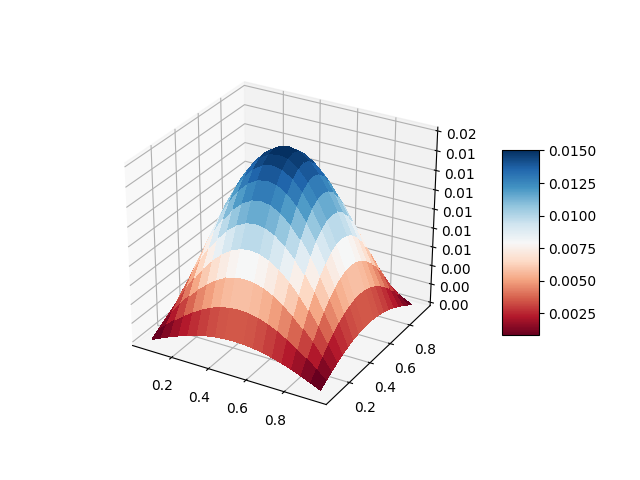
\includegraphics[width=10cm, height=10cm]{Opti.png}
    \caption{Estado Óptimo}
    \label{fig:my_label}
\end{figure}

\noindent
En la práctica este método no es muy usado debido a su lentitud de convergencia, por lo cual se usan versiones análogas de estos métodos, como el método de Newton para resolverlo. 
\subsection{Primero discretizar, luego optimizar}
Este método consiste primero en discretizar todo en el problema 26 para obtener un problema de optimización cuadrática de finitas variables y resolverlo para obtener una aproximación de la solución. En este caso, el problema se discretizó igual que antes con un esquema de diferencias finitas, en una malla cuadricular de tamaño $50\times 50$ . En particular, se reemplazó el término del Laplaciano por la aproximación
\begin{equation}
\Delta y\approx \frac{1}{h^{2}}\left(-y_{i+1, j}+2 y_{i, j}-y_{i-1, j}-y_{i, j+1}+2 y_{i, j}-y_{i, j-1}\right)
\end{equation}
y la función se evaluaron todas las funciones en los puntos de la malla. Después de discretizar todo y usando orden lexicográfico para ordenar las variables, obtenemos el problema en finitas variables 
\begin{equation}
\begin{split}
  \min& \frac{h^2}{2} \sum_{i=1}^{(n-1)^{2}}\left[\left(y_{i}-y_{d,i}\right)^{2}+\lambda u_{i}^{2}\right]\\
  &\text{ s.t. } A_h \vec{y}= \Vec{u}
\end{split}
\end{equation}
Donde $\vec{u},\vec{y}$ son vectores de tamaño $(N-1)^2$ y $A_h$ es la matriz dada por 
\begin{equation}A_{h}=h^{-2}\left(\begin{array}{cccc}
B & -I & & \\
-I & B & \ddots & \\
& \ddots & \ddots & -I \\
& & -I & B
\end{array}\right)\end{equation}
donde $B$ es la matriz en $M_{(N-1)\times (N-1)}$
\begin{equation}B=\left(\begin{array}{cccc}
4 & -1 & & \\
-1 & 4 & \ddots & \\
& \ddots & \ddots & -1 \\
& & -1 & 4
\end{array}\right)\end{equation}
Este problema de optimización cuadrática se puede resolver con solvers existentes, en este caso usé cvxopt en python para resolverlo. El estado óptimo que obtuve fue muy parecido al que produjo el otro método.
\begin{figure}[H]
    \centering
    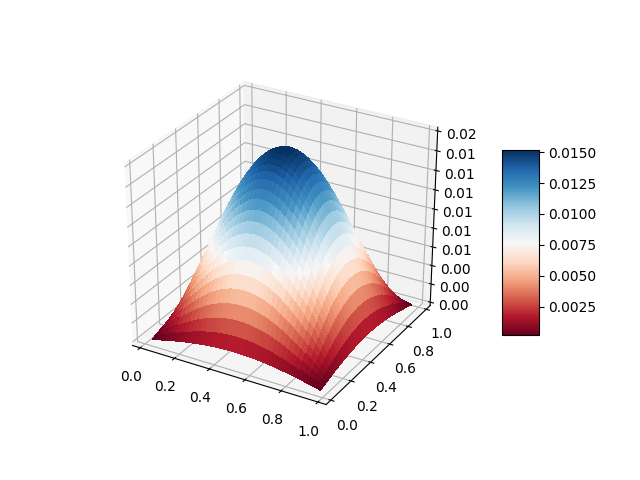
\includegraphics[width=10cm, height=10cm]{cuadratica.png}
    \caption{Estado Óptimo}
    \label{fig:my_label}
\end{figure}
\noindent
Este método es dependiente del mallado, algo poco deseable, por lo que en general se prefieren los métodos de primero optimizar y luego discretizar. Sin embargo, es sencillo de implementar y en casos sencillos como este proporciona buenos resultados.\\

\noindent
Para problemas con dominios más complicados, una discretización con elementos finitos también es posible en ambas formas de abordar el problema. Existen muchos algoritmos de optimización para este tipo de problemas, pero la mayoría se basan en los mismo principios que los tratados con este ejemplo. \\

\noindent
El código donde se encuentran implementados los métodos se encuentra en \url{https://github.com/CarlosContrerasQ12/ProyectoOptimizacion}








\nocite{*}
\bibliography{references}
\bibliographystyle{unsrt}
\end{document}
